Kap. 23, s.798 -836

Vi fortsetter der Uke11 slapp, med operasjonsforsterkere.

\subsection{Virtuelt nullpunkt}
  Den indre motstanden i en opamp er veldig stor.
Det vil si at det virtuelt sett ikke går strøm igjennom.

$$i_i \approx 0$$
Og derfor er også
$$v_i \approx 0$$

Det gjør at vi betrakter inngangen til opampen som et virtuelt nullpunkt.
Det gjør også at vi kan forenkle uttrykk hvor $i_i$ eller $v_i$ inngår.

\subsection{Ikke-inverterende forsterker}
  I en ikke-inverterende forsterker er \emph{ikke} signalet faseforskjøvet 90°,
som i en inverterende forsterker.

\begin{figure}[H]
  \caption{Ikke-inverterende forsterker}
  \centering
  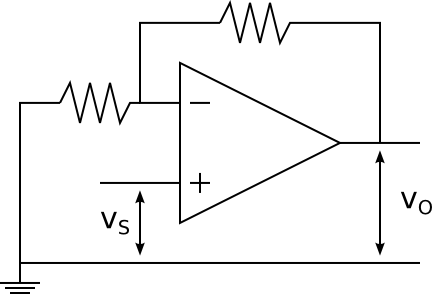
\includegraphics[width=0.5\textwidth]{./img/ikkeinv}
\end{figure}

$$v_O = \frac{R_1+R_2}{R_2} \cdot v_S
= \left( \frac{R_1}{R_2} + 1 \right) \cdot v_S$$

$$A_{vf} = \frac{v_O}{v_S} = \frac{R_1}{R_2}+1$$



\paragraph{Spenningsfølger} \mbox{} \\
Hvis $R_1$ eller $R_2$ er null blir forsterkningen 1.
Dette kalles en spenningsfølger.
Utgangen kan drive mer strøm enn kilden kan.
De kan brukes som "front end" til måleinstrumenter.

\subsection{Integratorkobling}
  Output av en integrator er integralet av input.
Det er ofte viktig å kalibrere signalet så det svinger presist rundt null,
ellers blir integralet feil.

\begin{figure}[H]
  \caption{Integratorkobling}
  \centering
  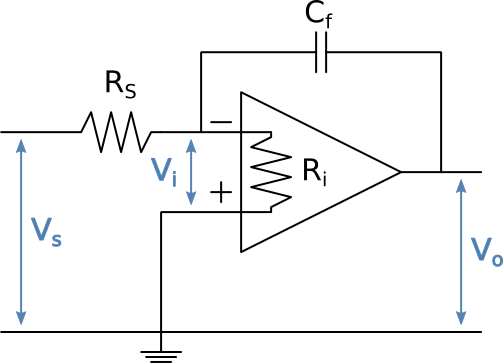
\includegraphics[width=0.5\textwidth]{./img/integrator}
\end{figure}



\paragraph{Strøm} \mbox{} \\
$$i_s = i_i + i_f$$
$$\frac{v_s - v_i}{R_s} = \frac{v_i}{R_i} + i_f$$



\paragraph{Spenning} \mbox{} \\
$$\frac{v_s}{R_s} = -C \cdot \frac{dv_o}{dt}$$
Løs med hensyn på $v_o$ og integrer på begge sider (Husk at $R_s$ og $C$
er konstanter).
$$v_o = -\frac{1}{R_sC} \int_0^t v_s dt$$

\subsection{Addisjon med OpAmp}
  Hver av signalene på input slås sammen før dem går inn i opampen.
I følgende krets har input forskjellig motstand, men de kan like så godt
ha samme motstand.
Lik motstand kan f.eks. brukes i et miksebord for lyd.
Ulik motstand kan brukes, som i bildet, til å konvertere binær til analog.

\begin{figure}[H]
  \caption{Addisjon med opamp}
  \centering
  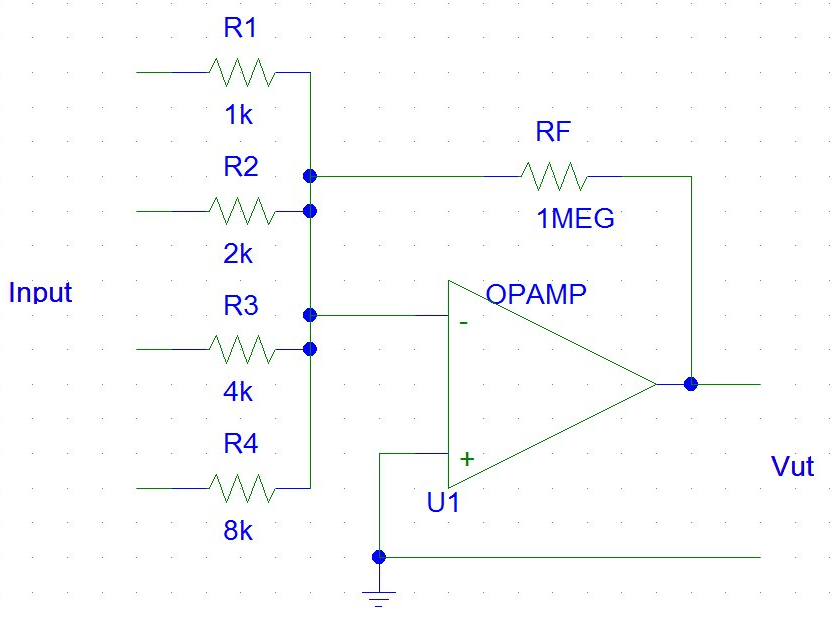
\includegraphics[width=0.67\textwidth]{./img/addisjon.png}
\end{figure}

Strømmen inn i knutepunktet er lik strømmen ut av det.
$$i_1 + i_2 + i_3 + i_4 = i_f + i_i$$
$$v_i \approx = 0 \rightarrow i_i = 0$$
Det gir at
$$\frac{v_1}{R_1} + \frac{v_2}{R_2} + \frac{v_3}{R_3} + \frac{v_4}{R_4}
  = -\frac{v_o}{R_f} \rightarrow v_o
  = -\left( v_1\frac{R_f}{R_1} +...+ v_4\frac{R_f}{R_4} \right)$$

Leddene $\frac{R_f}{R_n}$ kalles vekt og avgjør hvor mye hver av inputene skal
telle med i resultatet.
For et miksebord kan justering av channel gain endre på en slik vekt.
Master volumet kan justeres ved $R_f$.

\subsection{Differensial forsterker}
  En differensial opamp har signal på begge input.

\begin{figure}[H]
  \caption{Differensial OpAmp}
  \centering
  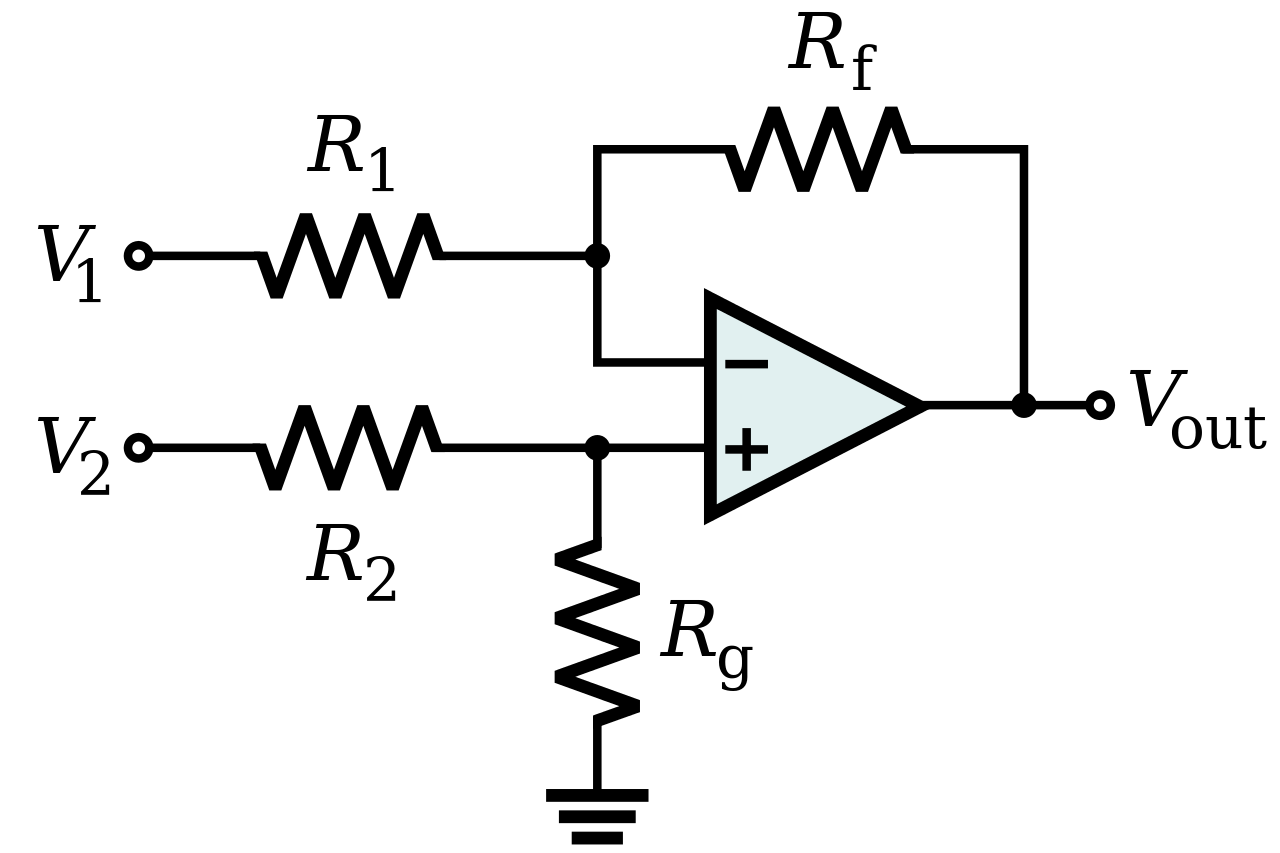
\includegraphics[width=0.5\textwidth]{./img/diffamp}
\end{figure}

For å finne $v_o$ bruker man superposisjonsprinsippet.
\\\\
$v_1$ alene $(v_2 = 0)$
$$v_{o1} = -\frac{R_f}{R_1} \cdot v_1$$

$v_2$ alene $(v_1 = 0)$
$$v_{o2} = \frac{R_f + R_1}{R_1} \cdot v_g$$
$$v_g = \frac{R_g}{R_2 + R_g} \cdot v_2$$
$$v_{o2} = \frac{R_f+R_1}{R_1} \cdot \frac{R_g}{R_2+R_g} \cdot v_2$$

Summen av bidragene
$$v_o = v_{o1} + v_{o2} =
  -\frac{R_f}{R_1}v_1 + \frac{(R_f+R_1)R_g}{R_1(R_2+R_g)}v_2$$

\subsection{Eksponential forsterker}
  \begin{figure}[H]
  \caption{Eksponensiell forsterker}
  \centering
  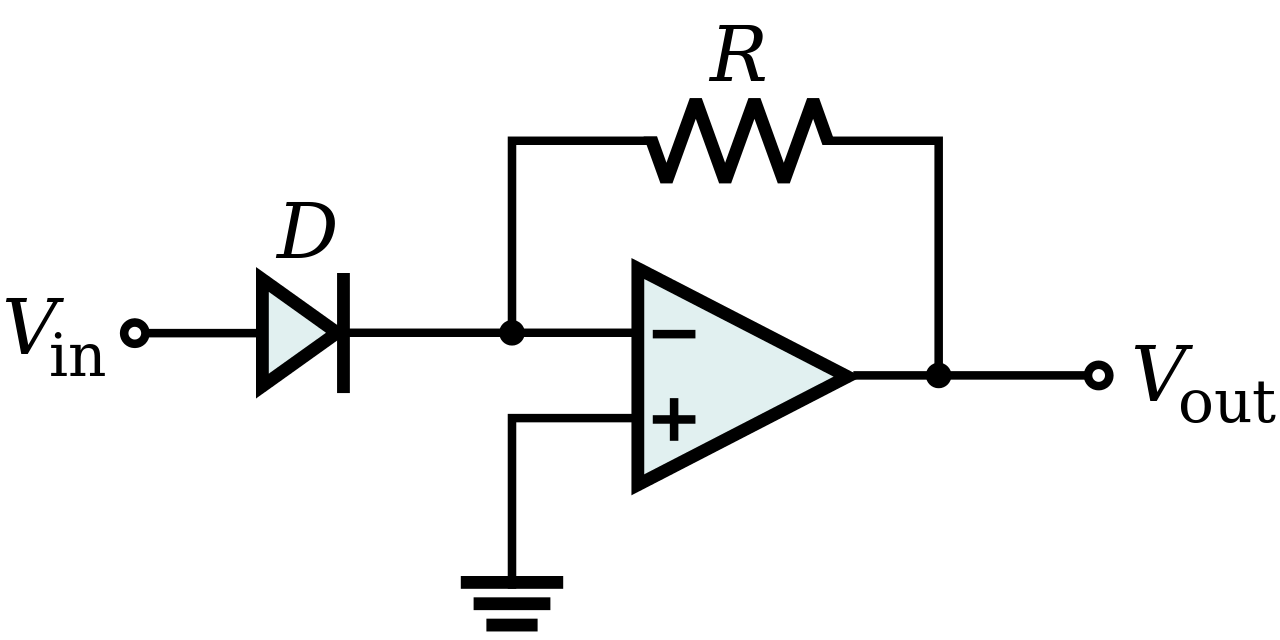
\includegraphics[width=0.5\textwidth]{./img/expamp}
\end{figure}

Spenningen ut er gitt ved
$$v_o = -R_f \cdot i_f \approx -R_f \cdot I_s \cdot e^{\frac{V_s}{V_T}}$$

\subsection{Logaritmisk forsterker}
  Hvis man, med utgangspunkt i eksponensiell forsterker, bytter plasseringen
til motstanden og dioden får man en logaritmisk forsterker.

\begin{figure}[H]
  \caption{Logaritmisk forsterker}
  \centering
  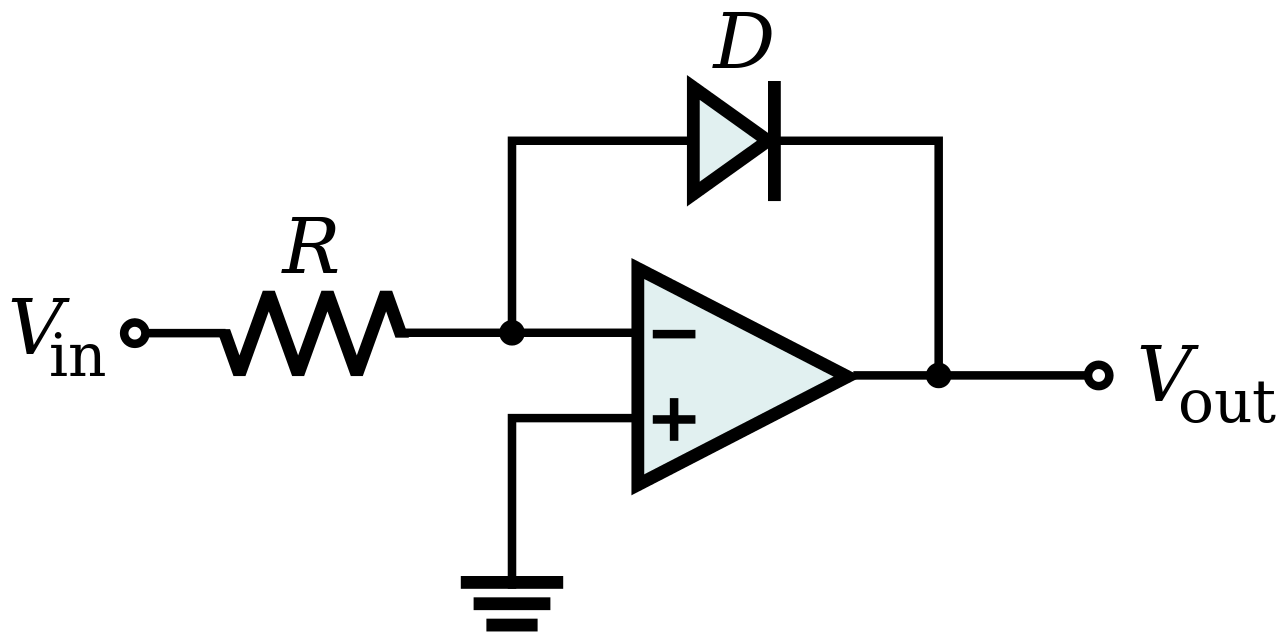
\includegraphics[width=0.5\textwidth]{./img/logamp}
\end{figure}

Spenningen ut er gitt ved
$$v_o = -V_T \cdot \ln{v_s}$$

\subsection{Frekvensforløp}
  Opampens forsterkning begrenses av høy frekvens.
Et Bode-diagram viser sammenhengen mellom fekvens og forsterkning.
\\\\
Signalet til en opamp blir også faseforskjøvet etter som frekvens endrer seg.
For hver 2. dekade blir signalet forskjøvet med 90°.

\begin{figure}[H]
  \caption{Forhold mellom forsterkning/fase og frekvens}
  \centering
  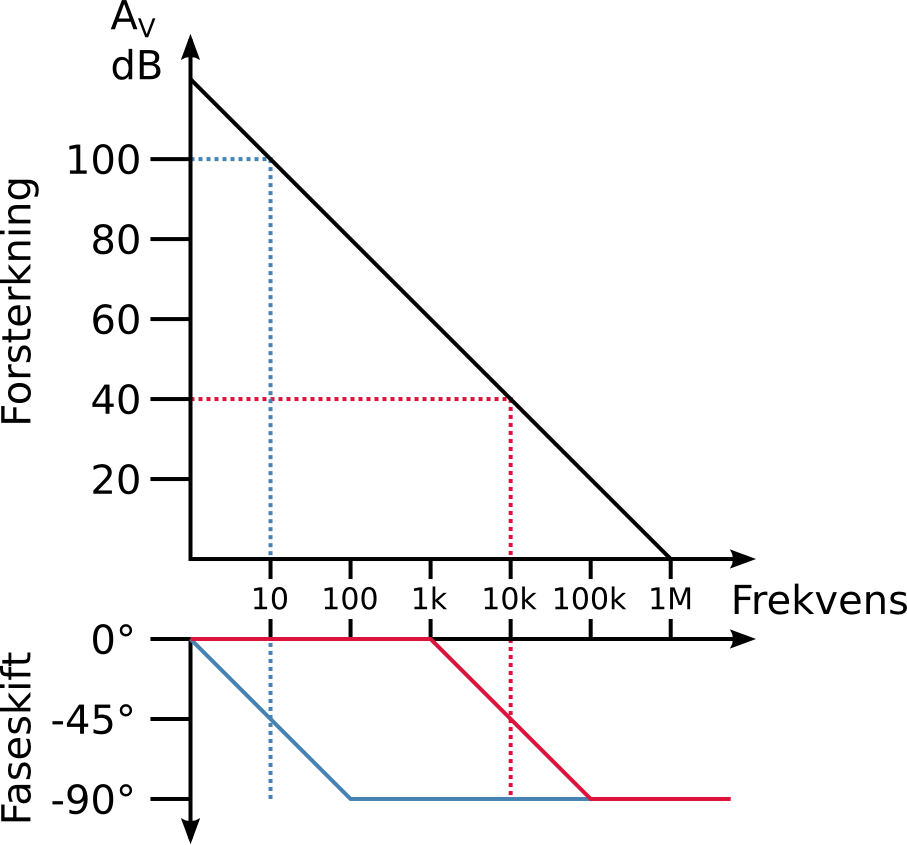
\includegraphics[width=0.67\textwidth]{./img/frekfor}
\end{figure}

Båndbredden er avhengig av hvilken forsterkning vi ønsker.
F.eks. vil $A_v = 40dB$ gi en øvre grense på 10kHz.
Og forsterkning på 20dB har øvre grense på 100kHz.
\\\\
Ved grensefrekvensen forekommer et faseskifte.
Som man kan se begynner det én dekade før og ender én dekade etter.
Totalt 90° forskyvning.



\paragraph{Gain-Bandwidth Product} \mbox{} \\
Gain-Bandwidth Product, GBW, bestemmer skråningen på grafen over.
Produsenter oppgir GBW ved $A_v = 1$, altså der grafen treffer x-aksen.
\\\\
Eksempel\\
$$GBW = A_v \cdot B_w$$
La oss si at $GBW = 1MHz$ og vi ønsker forsterkning på $A_v = 100$.
$$BW = \frac{1MHz}{100} = 10kHz$$

